\chapter{QuadTree on celestial sphere}
\label{cha:quadtree}
%
\note{Improve the description of the quadtree, its construction etc\ldots}
%
\section{Introduction}
%
The extraction of galaxy groups from the redshift space implies in all kind
of algorithms to search for galaxies in a given region of the sky. Methods
as those used in numerical simulations for searching dark matter halos
should be applied. Such techniques often use a partition of the space to
make a brute force computation of the distance between particles only on a
small portion of the three dimensional space. Same partitioning of the
celestial sphere can be done, but the non-euclidean metric of celestial
coordinates make the task a little harder.
%
\section{QuadTree}
%
The principle of the QuadTree is to make a partition of the space (celestial
sphere in our case). Each created partition will be partitioned too if the
number of galaxies in it is superior to a limit we define at the creation of
the QuadTree. If the number of levels in the refinement is superior to a
given limit, we stop the refinement.

This is clearly a tree structure, since the partitions, called nodes, are
subdivided into other nodes. This allow to rapidly search for galaxies in a
given region since we can easily determine which node intersect a given
region.
%
\subsection{Construction}
%
The construction is straightforward with the description above. We start by
defining the limits in the $(\alpha, \delta)$ plane for the region to
refine. This region is the root node. Then the following instructions are
applied recursively.
%
\begin{itemize}
    \item We determine in which node each points, in the parent node, are
        falling inside. We keep an array of the identities of points in the
        tree to which each node point to. In this array, identities are
        ordered by nodes into the associated point belongs to. So, at the
        end of the tree construction, the array of the identities will
        structured in the same as the tree, allowing optimization of the
        memory and future search of points.
    \item If the maximal level of refinement is reached, we stop to subdivide
        the node.
    \item If the number of points in the child node is superior to the fixed
        limit, we subdivide the node in four other nodes.
    \item Go to the brother of the node.
\end{itemize}
%
For optimization, we keep just nodes that are not empty, linking together
brother nodes.

During the construction of the node, we also keep informations on their
spatial geometry such as extremal coordinates in right ascension and
declination, center position, half width in each axis to avoid useless
computations when searching points on the celestial sphere.

At this stage, we make a simple partition of the space as in any other
QuadTree, without caring about the special metric involved.

An illustration of a QuadTree generated for the galaxies in the adjoining
block of the SDSS is shown in Figure~\ref{fig:quadtree}.
%
\begin{figure}
    \centering
    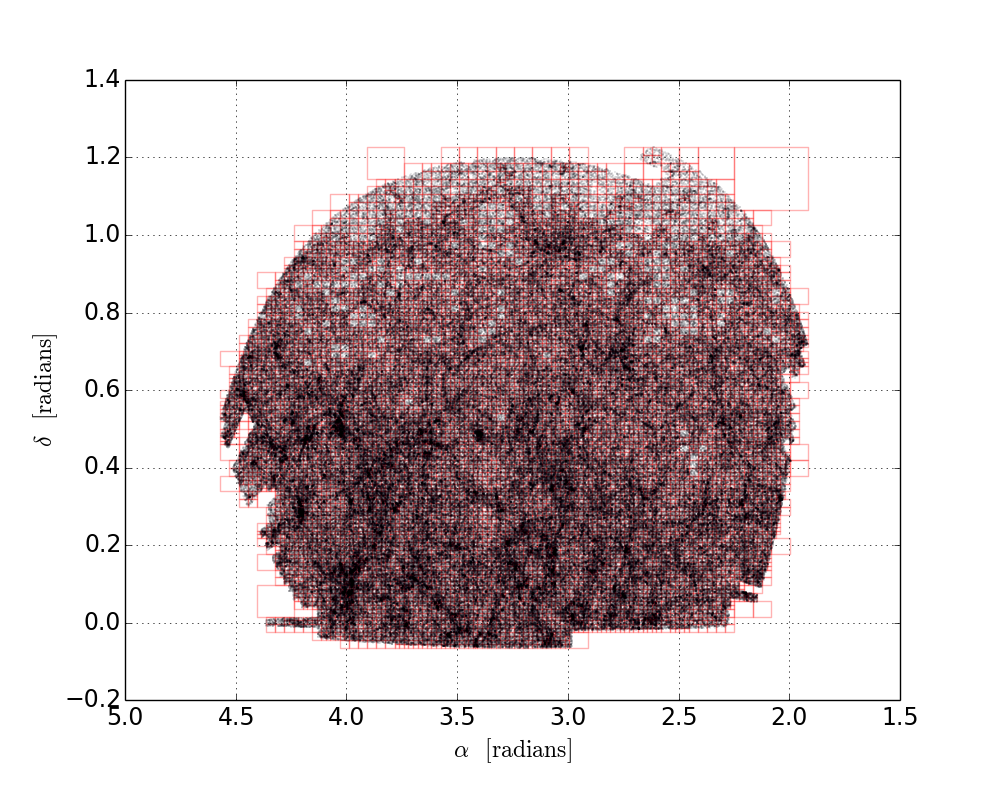
\includegraphics[width=0.7\linewidth]{figures/appendix/quadtree/quadtree.png}
    \caption{A simple illustration of a QuadTree generated for the SDSS
        adjoining block of galaxies. The tree is more refined in the dense projected
    region on the sky.\label{fig:quadtree}}
\end{figure}
%
\subsection{Searching in a given region}
%
To search in a given region, we go recursively through the tree structure, finding all
nodes that intersect it. An improvement can be done by computing if a node
is entirely contained by the searching region. If yes, we can directly use
the pointer to the identities array to include its points, without
descending more in the tree.

Defining if the region and a node intersect is easy since they are defined
as two rectangles in a two dimensional space.

The rectangular region is defined in the declination axis simply by taking
the central declination coordinate and adding it the angular distance for
the research region, since no distortions are present along this axis. For
the right ascension, we need to know the maximal separation between the
central point and the spherical circle generated by the angular distance.
For this extremal case point, it is clear that the corresponding meridian is
tangent to the spherical circle. So, in the spherical triangle formed by our
central point, the extremal point and the pole, we have a supplementary
constraint. The sinus formula applied to it gives us:
%
\begin{equation}
    \Delta\alpha = \mathrm{asin}\left(\cfrac{\sin d}{\cos\delta_0}\right)
\end{equation}
%
where $d$ is the angular radius inside which we are searching for points and
$\delta_0$ is the declination of the central point around which we search.
Our rectangular area is completely defined, and the intersections with the
nodes of the tree are easy to compute.

The case of the periodic search is complex. If the rectangular region fall
outside the periodic limits (inferior to 0 or superior to $2\pi$ in right
ascension on the celestial sphere), we nedd to duplicate the search region
and make the intersection with nodes for two regions instead of one. This is
a little time consuming but is the only way to handle correctly the periodic
case.
%
\subsection{$k$ nearest neighbors}
%
The $k$ nearest neighbors in the celestial sphere uses the implementation of
the search in a given region of the sky.

We find the leaf node to which our central point belongs to. A particular
attention must be done since we keep only non empty nodes. If the point
belongs to an empty one, we affect to it the parent node. In each case, we
take the parent node of the found node and search points inside it. Their
identities are added to a queue of size $k$ in ascending order of distance
to the central point.

We define a search region with this most distant point and fill again the
queue with points of this region. If the number of points found is inferior
to $k$, we take the parent node and redo the same computation until the
queue is entirely filled with the $k$ nearest neighbors.
